% Author: Seongjin Lee
% Hanyang University, Seoul, Korea
% esos.hanyang.ac.kr
% 2016-09-20
% note: some slides are adopted from  \url{www.cs.stevens.edu/~jschauma/631A/}
% https://github.com/resourceful/lecture_sysprog/

\documentclass[newPxFont,sthlmFooter,nooffset]{beamer}
\usepackage{kotex}
%\usetheme{sthlm}
\usepackage{../beamer_template/beamerthemesthlm}
\hypersetup{pdfauthor={Seongjin Lee (insight@gnu.ac.kr)},
            pdfsubject={Lecture Note: System Programming},
            pdfkeywords={Lecture Note, System Programming, class, (under)graduate},
            pdfmoddate={D: \pdfdate},
            pdfcreator={Seongjin Lee}}

%\setbeamertemplate{footline}[text line]{%
%    \parbox{\linewidth}{\vspace*{-8pt} \insertsectionhead  \hfill\insertshortauthor\hfill\insertpagenumber}}
%\setbeamertemplate{navigation symbols}{}

\newcommand\Fontvi{\fontsize{10}{11}\selectfont}



\title{System Programming}
\subtitle{Week 4: Files and Directories}
\author[SJL]{Seongjin Lee}
\institute{\href{mailto:insight@gnu.ac.kr}{insight@gnu.ac.kr}\\\url{http://open.gnu.ac.kr}\\Systems Research Lab.\\Gyeongsang National University}
\date{\today}

\begin{document}



\frame[plain]{\titlepage}

\frame{\frametitle{Table of contents}\tableofcontents}


%---------------------------------------------------------

\begin{frame}[t]
  \frametitle{introduction}
Additional features of the file system and the properties of a file
\begin{itemize}
\item \texttt{stat} function and its structure
\item modifying the attributes: Owner, Permissions, etc.
\item \textsc{Unix} file system structure and symbolic links
\item functions that operate on directories
\end{itemize}
\end{frame}

\section{stat structures}

\begin{frame}[containsverbatim,t]
  \frametitle{stat and Related Functions}
\begin{codedef}
#include <sys/stat.h>
int stat(const char *restrict pathname, struct stat *restrict buf );
int fstat(int fd, struct stat *buf);
int lstat(const char *restrict pathname, struct stat *restrict buf );
int fstatat(int fd, const char *restrict pathname, struct stat *restrict buf, int flag);
&&\hfill // All four return: 0 if OK, −1 on error
\end{codedef}
\begin{itemize}
\item \texttt{stat}: returns a structure of information about the file
  at \textit{pathname}

\item \texttt{fstat}: obtains information about the file that is already
  open on the descriptor \texttt{fd}

\item \texttt{lstat}: returns info about the symbolic link, not the file
  referenced by the symbolic link

\item \texttt{fstatat} returns the file statistics for a pathname relative
  to an open directory represented by the \texttt{fd}
\end{itemize}
\end{frame}

\begin{frame}[containsverbatim,t]
  \frametitle{Definition of the stat Structure}
\begin{codedef}
struct stat {
   mode_t	st_mode;	/* file type & mode (permissions) */
   ino_t	st_ino;	/* i-node number (serial number) */
   dev_t	st_dev;	/* device number (file system) */
   dev_t	st_rdev;	/* device number for special files */
   nlink_t	st_nlink;	/* number of links */
   uid_t	st_uid;	        /* user ID of owner */
   gid_t	st_gid;	        /* group ID of owner */
   off_t	st_size;	/* size in bytes, for regular files */
   struct timespec st_atim;	/* time of last access */
   struct timespec st_mtim;	/* time of last modification */
   struct timespec st_ctim;	/* time of last file status change */
   blksize_t       st_blksize; /* best I/O block size */
   blkcnt_t        st_blocks;  /* number of disk blocks allocated */
};
\end{codedef}

Note that most members of the \texttt{stat} structure are specified by a \textit{primitive system data type} (see Section 2.8, header \texttt{<sys/types.h>})
\end{frame}

\begin{frame}[t]
  \frametitle{File Types}
Everything is a file in \textsc{Unix}. There are ....
\begin{itemize}
\item Regular file: {\footnotesize The most common type, and there is
    no disctiction whether the data is text or binary. Application is
    responsible for interpreting}
\item Directory file: {\footnotesize A file that contains the name of
    other files and pointers to information on these files. Any
    process can read, only kernel can write.}
\item Block sepcial file: {\footnotesize A type of file providing
    buffered I/O access in fixed-size units to devices such as disk
    drives}
\item Character special file: {\footnotesize A type of file providing
    unbuffered I/O access in variable-sized units to devices}
\item FIFO: {\footnotesize A Type of file used for communication
    between processes}
\item Socket: {\footnotesize A type of file used for network
    communication between processes}
\item Symbolic Link: {\footnotesize A type of file that points to another file}
\end{itemize}
\end{frame}

\begin{frame}[containsverbatim,t]
  \frametitle{File Types Cnt'd}
The type of a file is encoded in the \texttt{st\_mode} member of the \texttt{stat} structure

\begin{codedef}
struct stat st;
if (S_ISREG(st.st_mode));
    printf("Regular File\n");
\end{codedef}


\begin{center}
  \begin{table}
    \centering
    \begin{tabular}[t]{c | c}
    Macro & Type of file \\ \hline
    \texttt{S\_ISREG()}	&	regular file	\\  \hline
    \texttt{S\_ISDIR()}	&	directory file	\\  \hline
    \texttt{S\_ISCHR()}	&	character special file	\\  \hline
    \texttt{S\_ISBLK()}	&	block special file	\\  \hline
    \texttt{S\_ISFIFO()}	&	pipe or FIFO	\\  \hline
    \texttt{S\_ISLNK()}	&	symbolic link	\\  \hline
    \texttt{S\_ISSOCK()}	&	socket 	\\
  \end{tabular}
  \caption{File type macros in \texttt{<sys/stat.h>}}
\end{table}

\end{center}

\end{frame}

\begin{frame}[containsverbatim,t]
  \frametitle{File Types Cnt'd}
First, let's review \texttt{./codes/myls.c}
  \lstinputlisting[linerange={17,33},lineskip=-5pt]{./codes/myls.c}
\end{frame}

\begin{frame}[t]
  \frametitle{Let's improve the code (myls.c, Fig. 4.3)}
The code at the moment does not show file types.

Make changes to the code such that it prints out the file types.

Use Fig. 4.3 as reference.

\end{frame}

\section{Attributes}

\begin{frame}
  \frametitle{Set-User-ID and Set-Group-ID}
Every process has six or more IDs associated with it
  \begin{table}[h]
    \centering
    \begin{tabular}{l | l}
     real user ID & \multirow{2}{*}{who we really are} \\
     real group ID & \\ \hline
     effective group ID & \multirow{3}{*}{used for file accessed permission checks} \\
     effective group ID & \\
     supplimentary group IDs & \\ \hline
     saved set-user-ID & \multirow{2}{*}{saved by exec function} \\
     saved set-group-ID & \\
    \end{tabular}
    \caption{User IDs and group IDs associated with each process}
    \label{tab:uid_gid}
  \end{table}
Every file has an owner and a group owner. The owner is specified by the \texttt{st\_uid} member of the stat structure; the group owner, by the \texttt{st\_gid} member.
\end{frame}


\begin{frame}[t]
  \frametitle{File Access Permissions}
\Fontvi
  \begin{columns}[T]
    \begin{column}{0.4\textwidth}
      \begin{table}[h]\label{fig:4.6}
        \centering
        \begin{tabular}{l | l}
          st\_mode mask & Meaning \\ \hline
          S\_IRUSR & user-read   \\
          S\_IWUSR & user-write  \\
          S\_IXUS  & user-excute \\ \hline
          S\_IRGRP & group-read   \\
          S\_IWGRP & group-write  \\
          S\_IXGRP & group-excute \\ \hline
          S\_IROTH & other-read   \\
          S\_IWOTH & other-write  \\
          S\_IXOTH & other-excute \\
        \end{tabular}
        \caption{The nine file access permission bits from <sys/stat.h>}
        \end{table}
    \end{column}
    \begin{column}{0.6\textwidth}
      \begin{itemize}
      \item To open a file, need execute permission on each directory
        component of the path
      \item To open a file with \texttt{O\_RDONLY} or
        \texttt{O\_RDWR}, need read permission
      \item To open a file with \texttt{O\_ WRONLY} or
        \texttt{O\_RDWR}, need write permission
      \item To use \texttt{O\_TRUNC}, must have write permission
      \item To create a new file, must have write+execute permission
        for the directory
      \item To delete a file, need write+execute on directory, file
        doesn’t matter To execute a file (via exec family), need
        execute permission
      \end{itemize}
    \end{column}
  \end{columns}

\end{frame}

\begin{frame}[containsverbatim,t]
  \frametitle{access and faccessat Function}
When we open a file, the kernel performs its access tests based on the effective user and group IDs

  \begin{codedef}
 #include <unistd.h>
int access(const char *pathname, int mode);
int faccessat(int fd, const char *pathname, int mode, int flag);
\\ Both return: 0 if OK, −1 on error
  \end{codedef}
\bigskip
Tests file accessibility on the basis of the {\em real} \texttt{uid} and \texttt{gid}. It is useful when a process is running as someone else, using either the set-user-ID or set-group-ID feature

\begin{center}
  \begin{tabular}{c | c}
    \texttt{R\_OK} & test for read permission \\
    \texttt{W\_OK} & test for write permission \\
    \texttt{X\_OK} & test for execute permission \\
    \texttt{F\_OK} & test for existence of file \\
  \end{tabular}
\end{center}

\end{frame}



\begin{frame}[containsverbatim,t]
  \frametitle{access Function Example}
Let's review \texttt{codes/access.c}
\lstinputlisting[linerange={9,24},lineskip=-5pt]{codes/access.c}

\end{frame}



\begin{frame}[containsverbatim,t]
  \frametitle{access Function Example}
The steps are as follows
  \begin{enumerate}[ ]
  \item cd codes/ ; make access
  \item \texttt{ls -l access}
  \item \texttt{ls -l /etc/shadow}
  \item \texttt{./access /etc/shadow}
  \item \texttt{su chown root access}
  \item \texttt{chmod u+s access}
  \item \texttt{ls -l access}
  \item \texttt{./access /etc/shadow}
  \item \texttt{exit}
  \item \texttt{access /etc/shadow}
  \end{enumerate}
\end{frame}

\begin{frame}
  \frametitle{Order of Permission Tests}
Which permission set to use is determined (in order listed):
\begin{enumerate}
\item If effective-uid == 0 (the superuser), grant access
\item If effective-uid == \texttt{st\_uid} (the owner ID)
   \begin{enumerate}
   \item if appropriate user permission bit is set, grant access (user
     permissions are RWX)
   \item else, deny access
   \end{enumerate}
\item If effective-gid == \texttt{st\_gid} (the group ID)
   \begin{enumerate}
   \item if appropriate group permission bit is set, grant access
   \item else, deny access
   \end{enumerate}
\item If appropriate other permission bit is set, grant access, else deny access
\end{enumerate}
\end{frame}



\begin{frame}[containsverbatim,t]
  \frametitle{umask Function}
Every process has file mode creation mask

\begin{codedef}
#include <sys/stat.h>
mode_t umask(mode_t cmask);
// Returns: previous file mode creation mask
\end{codedef}

\textit{cmask} argument is formed as the bitwise OR of the nine constants from page \ref{fig:4.6}
\end{frame}


\begin{frame}[containsverbatim,t]
  \frametitle{umask Example}
Let's review \texttt{codes/myumask.c}
\lstinputlisting[linerange={10,26}, lineskip=-5pt]{./codes/myumask.c}
\end{frame}


\begin{frame}[containsverbatim,t]
  \frametitle{umask Example}
{\footnotesize
\begin{verbatim}
James@maker$ umask
0022
James@maker$ ./umask
James@maker$ ls -l foo bar
-rw-------  1 James  staff  0 Sep 25 23:06 bar
-rw-rw-rw-  1 James  staff  0 Sep 25 23:06 foo
James@maker$
\end{verbatim}
}
\end{frame}

\begin{frame}[t]
  \frametitle{umask More}
Most users on \textsc{Unix} systems never deal with their \texttt{umask} value (set only once, on login, by the shell's start-up file, and never changed).
\bigskip

If you want to ensure that specific access permission bits are enabled, you must modify the \texttt{umask} value while your process is running.

\end{frame}



\begin{frame}[containsverbatim,t]
    \frametitle{chmod, fchmod, and fchmodat Functions}
\begin{codedef}
#include <sys/stat.h>
int chmod(const char *pathname, mode_t mode);
int fchmod(int fd, mode_t mode);
int fchmodat(int fd, const char *pathname, mode_t mode, int flag);
// All three return: 0 if OK, −1 on error
\end{codedef}
\bigskip

\begin{itemize}
\item The \texttt{chmod} function operates on the specified file
\item \texttt{fchmod} function operates on a file that has already been opened
\item \texttt{fchmodat} function behaves like \texttt{chmod} when the \textit{pathname}  arguments is absolute or when the \textit{fd} argument has the value \texttt{AT\_FDCWD} and the \textit{pathname} argument is relative
\end{itemize}
\end{frame}


\begin{frame}
  \frametitle{chmod, fchmod, and fchmodat Functions}

{\footnotesize
\begin{table}[t]
\centering
\begin{tabular}[t]{l | l }
mode 	&	Description 	\\ \hline
S\_ISUID	&	set-user-ID on execution 	\\ \hline
S\_ISGID	&	set-group-ID on execution 	\\ \hline
S\_ISVTX	&	saved-text (sticky bit) 	\\ \hline
S\_IRWXU	&	read, write, and execute by user (owner) 	\\ \hline
~~~   S\_IRUSR	&	read by user (owner)	\\ \hline
~~~   S\_IWUSR	&	write by user (owner)	\\ \hline
~~~   S\_IXUSR	&	execute by user (owner) 	\\ \hline
S\_IRWXG	&	read, write, and execute by group 	\\ \hline
~~~   S\_IRGRP	&	read by group	\\ \hline
~~~   S\_IWGRP	&	write by group	\\ \hline
~~~   S\_IXGRP	&	execute by group 	\\ \hline
S\_IRWXO	&	read, write, and execute by other (world) 	\\ \hline
~~~   S\_IROTH	&	read by other (world)	\\ \hline
~~~   S\_IWOTH	&	write by other (world)	\\ \hline
~~~   S\_IXOTH	&	execute by other (world) 	\\ \hline
\end{tabular}
\caption{the mode constants for chmod function from <sys/stat.h>}
\label{tab:fig:4.11}
\end{table}
}

\end{frame}




\begin{frame}[t]
    \frametitle{chmod, fchmod, and fchmodat Functions}
\begin{block}{To change the permission bits of a file}
The effective user ID of the process must be equal to the owner ID of the file (\texttt{uid = st\_uid}), or the process must have superuser permissions
\end{block}

The \textit{mode} is specified as the bitwise OR of the constraints showns in the table
\bigskip

Note that nine of the entries are the nine file access permission bits from Page \ref{fig:4.6}

\end{frame}

\begin{frame}[containsverbatim,t]
  \frametitle{chmod Example}
Let's review \texttt{codes/mychmod.c}
\lstinputlisting[linerange={13,31},lineskip=-5pt]{codes/mychmod.c}
\end{frame}

\begin{frame}[fragile,containsverbatim,t]
  \frametitle{chmod Example}
\begin{verbatim}
James@maker:codes$ umask 077
James@maker:codes$ touch foo bar
James@maker:codes$ chmod a+rx foo
James@maker:codes$ ls -l foo bar
-rwxr-xr-x  1 James  staff  0 Sep 26 00:04 foo
-rw-------  1 James  staff  0 Sep 26 00:04 bar
James@maker:codes$ make mychmod
cc -g -Wall -O0 -c mychmod.c
cc -g -Wall -O0 -o mychmod mychmod.o
James@maker:codes$ ./mychmod
James@maker:codes$ ls -al foo bar
-rwsr--r-x  1 James  staff  0 Sep 26 00:04 foo
-rw-r--r--  1 James  staff  0 Sep 26 00:04 bar
\end{verbatim}
\end{frame}


\begin{frame}[containsverbatim,t]
  \frametitle{chown, fchown, fchownat, and lchown Function}
The \texttt{chown} functions allow us to change a file’s user ID and group ID,

\bigskip
\begin{codedef}
#include <unistd.h>
int chown(const char *pathname, uid_t owner, gid_t group);
int fchown(int fd, uid_t owner, gid_t group);
int fchownat(int fd, const char *pathname, uid_t owner, gid_t group, int flag);
int lchown(const char *pathname, uid_t owner, gid_t group);
// All four return: 0 if OK, −1 on error
\end{codedef}
\end{frame}


\begin{frame}[t]
  \frametitle{chown, fchown, fchownat, and lchown Function}
If either of the arguments \textit{owner} or \textit{group} is −1, the corresponding ID is left unchanged

\bigskip
Non-superusers can change the \texttt{st\_gid} field if followings are true
\begin{itemize}
\item \texttt{effective-user ID == st\_uid}
\item \texttt{owner == file's user ID} and \texttt{group == effective-group ID}
\end{itemize}
\end{frame}





\begin{frame}[t]
  \frametitle{File Size}
\texttt{st\_size} member of the \texttt{stat} structure contains the size of the file in bytes
\begin{itemize}
\item Regualr file -- a file size of 0 is allowed; returns end-of-file indications on the first read of the file
\item Directory -- the file size usually a multiple of a number
\item a symbolic link -- the file size is the number of bytes in the filename
\end{itemize}
\end{frame}


\begin{frame}[fragile,t]
  \frametitle{File Size Example}

Watch how the size of directory grows

\begin{verbatim}
mkdir -p /tmp/temp; ls -ld /tmp/temp
for file in a b c d e f g ; do
touch /tmp/temp/${file} ; echo "creating /tmp/temp/${file}"
ls -ld /tmp/temp;
done
\end{verbatim}

How about the size of symbolic link
\begin{verbatim}
DIRNAME=`pwd`
ln -s $DIRNAME /tmp/symlinkfile
ls -l /tmp/symlinkfile
echo $DIRNAME | wc -c
\end{verbatim}
\end{frame}

\begin{frame}[containsverbatim,t]
  \frametitle{File Truncation}
\begin{codedef}
#include <unistd.h>
int truncate(const char *pathname, off_t length);
int ftruncate(int fd, off_t length);
// Both return: 0 if OK, −1 on error
\end{codedef}
The two functions truncate an existing file to \textit{length} bytes.
\begin{itemize}
\item if the file is greater than \textit{length}, the data beyond \textit{length} is no longer accessible
\item Previous size was less than \textit{length}, the file size will increase, the in between data will read as \texttt{0}
\end{itemize}

\end{frame}


\section{File System Structures}


\begin{frame}
  \frametitle{Disk drive, partitions, and a file system}
We can think of a disk drive being divided into one or more partitions. Each partition can contain a file system. The i-nodes are fixed-length entries that contain most of the information about a file.
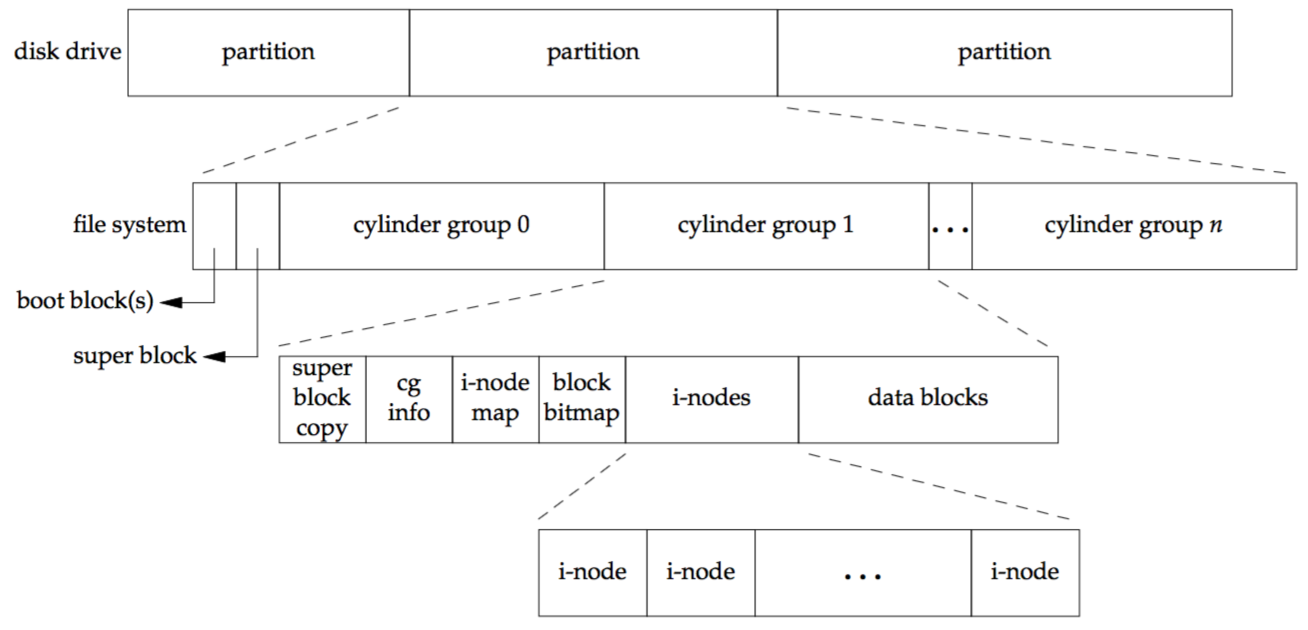
\includegraphics[width=\textwidth]{figure/fig4_13_disk.png}
\end{frame}



\begin{frame}
  \frametitle{Cylinder group's inodes and data blocks in more detail}
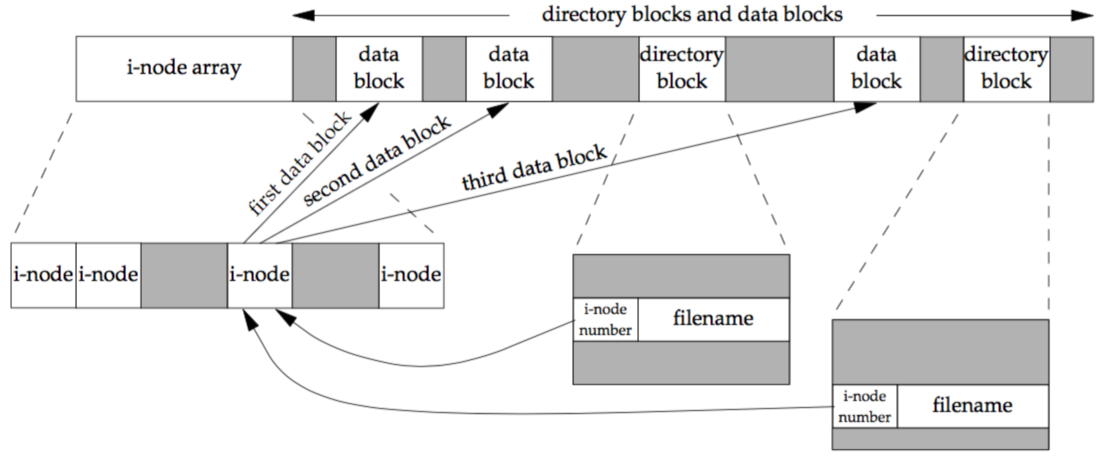
\includegraphics[width=\textwidth]{figure/fig4_14_cylinder.png}

Shows example of two directory entries point to the same i-node
  entry.
\end{frame}


\begin{frame}
  \frametitle{Cylinder group's inodes and data blocks in more detail}
  \begin{itemize}
  \item Every i-node has a link count that contains the number
    of directory entries that point to it. Only when the link count
    goes to to 0 can the file be deleted
  \item Symbolic link, the actual contents of the file--data blocks--
    store the name of the file that the symbolic link points to
  \item i-node contains all the information about the file
  \item data type for i-node number is \texttt{ino\_t}
  \item Only two items are in directory entry
    \begin{itemize}
    \item the filename
    \item the i-node number
    \end{itemize}
  \item directory entry can't refer to an i-node in a different File System
  \item When renaming, add a new directory entry that points to the existing i-node and then unlink the old directory entry
  \end{itemize}

\end{frame}

\begin{frame}
  \frametitle{Sample cylinder group after creating the directory testdir}
Result of \texttt{\$ mkdir testdir} ; the two entries ``dot'' and ``dot-dot''
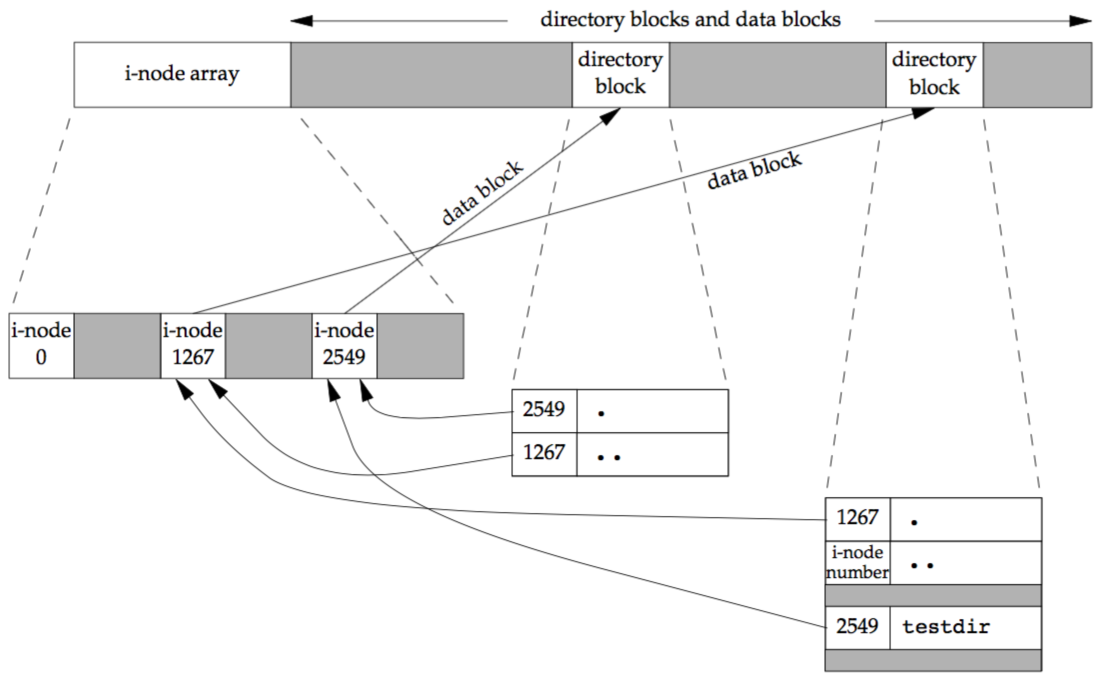
\includegraphics[width=\textwidth]{figure/fig4_15_sample.png}
\end{frame}



\begin{frame}[containsverbatim,t]
  \frametitle{link(2) Function}
\begin{codedef}
#include <unistd.h>
int link(const char *existingpath, const char *newpath);
int linkat(int efd, const char *existingpath, int nfd, const char *newpath, int flag);
// Both return: 0 if OK, −1 on error
\end{codedef}

{\footnotesize
\begin{itemize}
\item These functions create a new directory entry, \textit{newpath},
  that references the existing file \textit{existingpath}. If the
  \textit{newpath} already exists, an error is returned. Only the last
  component of the \textit{newpath} is created. The rest of the path
  must already exist.
\item With the \texttt{linkat} function, the existing file is specified by
  both the \textit{efd} and \textit{existingpath} arguments, and the
  new pathname is specified by both the \textit{nfd} and
  \textit{newpath} arguments.
\item When the existing file is a symbolic link, the flag argument controls the behavior
  \begin{itemize}
  \item \texttt{AT\_SYMLINK\_FOLLOW} flag -- link is created to the target of the symbolic link
  \item no flag -- link is created to the symbolic link itself
  \end{itemize}
  \item  Most implementations require that both pathnames be on the same file system
\end{itemize}
}

\end{frame}



\begin{frame}[containsverbatim,t]
  \frametitle{unlink(2) Function}
\begin{codedef}
#include <unistd.h>
int unlink(const char *pathname);
int unlinkat(int fd, const char *pathname, int flag);
// Both return: 0 if OK, −1 on error
\end{codedef}

{\footnotesize
\begin{itemize}
\item Remove the directory entry and decrement the link count of the file referenced by \textit{pathname}
\item If there are other links to the file, the data in the file is still accessible through the other links
\item To unlink a file, we must have write  and execute permission in the directory containing the directory entry because we are modifying the directory entry
\item Only when the link count reaches 0 can the contents of the file be deleted
\item If a process has the file open, its contents will not be deleted
  \begin{itemize}
  \item The kernel first checks the count of the number of processes that have the file open
  \item if this count has reaced \texttt{0}, the kernel then checks the link count
  \item if it is \texttt{0}, the file's contents are deleted
  \end{itemize}
\end{itemize}
}
\end{frame}

\begin{frame}[fragile]
  \frametitle{Open a file and then unlink it}
{\footnotesize
\begin{verbatim}
James@maker:codes$ make unlink
James@maker:codes$ df ~
Filesystem 512-blocks      Used Available Capacity  iused   ifree %iused  Mounted on
/dev/disk1  487830528 460268648  27049880    95% 57597579 3381235   94%   /
James@maker:codes$ ./myunlink &
[1] 11641
file unlinked
James@maker:codes$ df ~
Filesystem 512-blocks      Used Available Capacity  iused   ifree %iused  Mounted on
/dev/disk1  487830528 460268600  27049928    95% 57597573 3381241   94%   /
James@maker:codes$ done
[1]+  Done                    ./myunlink
James@maker:codes$ df ~
Filesystem 512-blocks      Used Available Capacity  iused   ifree %iused  Mounted on
/dev/disk1  487830528 459245352  28073176    95% 57469667 3509147   94%   /
\end{verbatim}
}
\end{frame}


\begin{frame}[t]
  \frametitle{Open a file and then unlink it}
  \begin{block}{Exploitation of unlink property}
  This property of unlink is often used by a program to ensure that a temporary file it creates won’t be left around in case the program crashes. The process creates a file using either open or creat and then immediately calls unlink. The file is not deleted, however, because it is still open. Only when the process either closes the file or terminates, which causes the kernel to close all its open files, is the file deleted.
  \end{block}
\end{frame}



\begin{frame}[containsverbatim,t]
  \frametitle{remove(2) Function}
\begin{codedef}
#include <stdio.h>
int remove(const char *pathname);
// Returns: 0 if OK, −1 on error
\end{codedef}

We can also unlink a file or a directory with the \texttt{remove} function. For a file, \texttt{remove} is identical to \texttt{unlink}. For a directory, \texttt{remove} is identical to \texttt{rmdir}.
\end{frame}

\begin{frame}[containsverbatim,t]
  \frametitle{rename Function}
File or a directory is renamed with either the \texttt{rename} or \texttt{renameat} function

\begin{codedef}
#include <stdio.h>
int rename(const char *oldname, const char *newname);
int renameat(int oldfd, const char *oldname, int newfd, const char *newname);
// Both return: 0 if OK, −1 on error
\end{codedef}

\end{frame}

\begin{frame}[t]
  \frametitle{rename Function - the detail}
\texttt{int rename(const char *oldname, const char *newname);}
\bigskip

If oldname refers to \textbf{is a file}, it is renaming a file or a symbolic link.
{\footnotesize
\begin{itemize}
\item
  \begin{itemize}
  \item If \textit{newname} exists and is not a directory, it is
    removed, and \textit{oldname} is renamed to \textit{newname}.
  \item w+x permission for directory containing \textit{oldname} and \textit{newname}
  \end{itemize}
\end{itemize}
}

\end{frame}


\begin{frame}[t]
  \frametitle{rename Function - the detail}

\texttt{int rename(const char *oldname, const char *newname);}
\bigskip

If oldname refers to \textbf{is a directory}, it is renaming a directory.

\begin{itemize}
\item if \textit{newname} exists and is an empty directory, it is
  removed; \textit{oldname} is renamedd \textit{newname}
\item if \textit{newname} exists and is a file, an error is returned
\item if \textit{oldname} is a prefix of \textit{newname}, an error is
  returned
\item w+x permission for directory containing \textit{oldname} and
  \textit{newname}
\end{itemize}

\end{frame}


\begin{frame}[t]
  \frametitle{rename Function - the detail}

\texttt{int rename(const char *oldname, const char *newname);}
\bigskip

Other details

\begin{itemize}
\item \textbf{\textit{oldname} or \textit{newname} is symbolic link},
  then the link itself is processed, not the file to which it resolves
\item We can’t rename dot or dot-dot.
\item As a special case, if \textit{oldname} and \textit{newname}
  refer to the same file, the function returns successfully without
  changing anything.
\end{itemize}

\end{frame}



\begin{frame}[containsverbatim,t]
  \frametitle{Creating Symbolic Links}

\begin{codedef}
#include <unistd.h>
int symlink(const char *actualpath, const char *sympath);
int symlinkat(const char *actualpath, int fd, const char *sympath);
// Both return: 0 if OK, −1 on error
\end{codedef}

\begin{itemize}
\item A new directory entry, \textit{sympath}, is created that points to \textit{actualpath}.
\item It is not required that \textit{actualpath} exist when the symbolic link is created.
\end{itemize}
\end{frame}


\begin{frame}[containsverbatim,t]
  \frametitle{Reading Symbolic Links}

Because the \texttt{open} function follows a symbolic link, we need a way to open the link itself and read the name in the link. The \texttt{readlink} and \texttt{readlinkat} functions do this.

\begin{codedef}
#include <unistd.h> ssize_t readlink(const char* restrict pathname, char *restrict buf, size_t bufsize); ssize_t
readlinkat(int fd, const char* restrict pathname, char *restrict buf, size_t bufsize);
// Both return: number of bytes read if OK, −1 on error
\end{codedef}
\end{frame}


\begin{frame}[t]
  \frametitle{File Times}

\begin{table}[t]
\centering
\begin{tabular}[t]{{l | l | l | l }}
Field & Description & Example & \texttt{ls(1) option} \\ \hline \hline
\texttt{st\_atim} & last-access time of file data & \texttt{read} & \texttt{-u} \\
\texttt{st\_mtim} & last-modification time of file data & \texttt{write} & default \\
\texttt{st\_ctim} & last-change time of i-node status & \texttt{chmod}, \texttt{chown} & \texttt{-c} \\
\end{tabular}
\caption{The three time values associated with each file}
\end{table}

\texttt{ls} command displays or sorts only on one of the three time values
\begin{itemize}
\item \texttt{-l} or \texttt{-t} : uses the modification time of a file
\item \texttt{-u} : uses the access time
\item \texttt{-c} : use the changed status time
\end{itemize}

\end{frame}

\begin{frame}[t]
  \frametitle{Effect of various functions on the \texttt{mac} times}
\centering
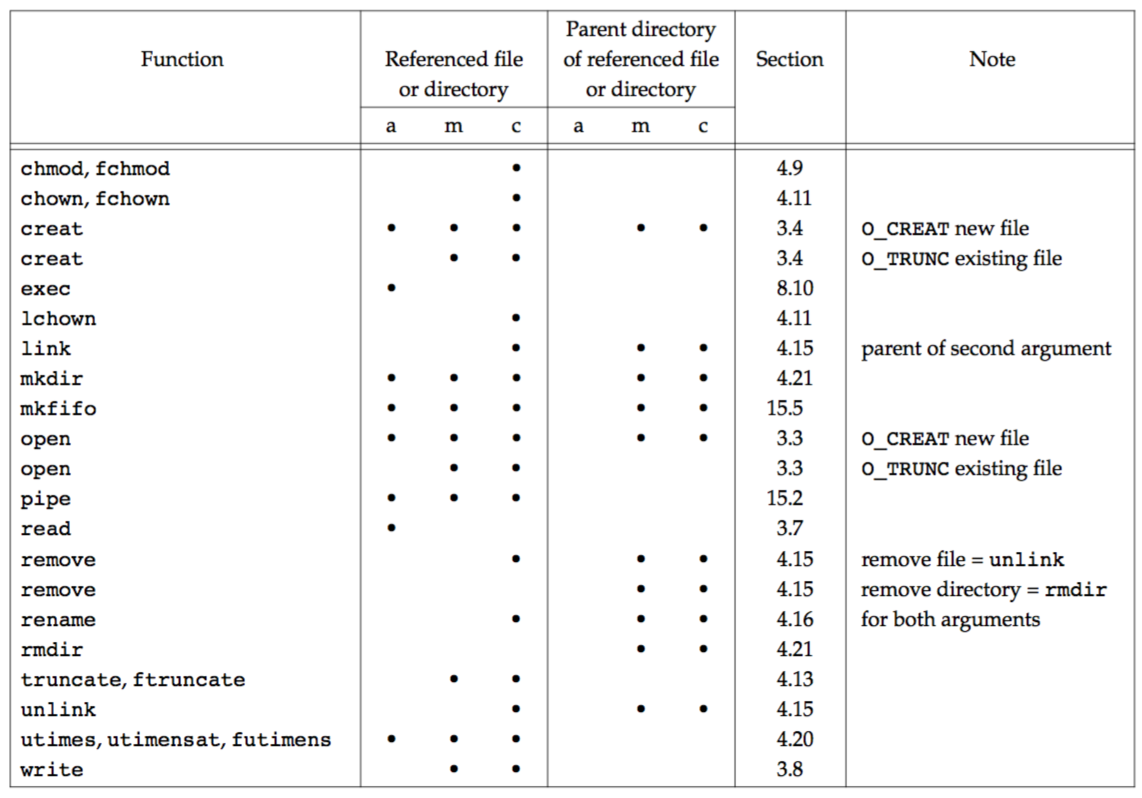
\includegraphics[height=0.90\textheight]{figure/fig4_20_effect.png}
\end{frame}



\begin{frame}[containsverbatim,t]
  \frametitle{futimens, utimensat, and utimes Functions}
Several functions are available to change the access time and the modification time of a file. The \texttt{futimens} and \texttt{utimensat} functions provide \textit{nanosecond} granularity for specifying timestamps, using the \texttt{timespec} structure
\bigskip

\begin{codedef}
#include <sys/stat.h>
int futimens(int fd, const struct timespec times[2]);
int utimensat(int fd, const char *path, const struct timespec times[2], int flag);
// Both return: 0 if OK, −1 on error
\end{codedef}
{\footnotesize
\begin{itemize}
\item If times is NULL, access time and modification time are set to
  the current time (must be owner of file or have write permission).
\item If times is non-NULL, then times are set according to the timeval
  struct array. For this, you must be the owner of the file (write
  permission not enough).  \bigskip
\item Note that \texttt{st\_ctime} is set to the current time in both
  cases.  \bigskip
\end{itemize}
}
\end{frame}

\begin{frame}[containsverbatim,t]
    \frametitle{futimens, utimensat, and utimes Functions}

\begin{codedef}
#include <sys/time.h>
int utimes(const char *pathname, const struct timeval times[2]);
// Returns: 0 if OK, −1 on error
\end{codedef}

The \texttt{utimes} function operates on a pathname. The \textit{times} argument is a pointer to an array of two timestamps — access time and modification time — but they are expressed in \textit{seconds} and \textit{microseconds}:

\begin{codedef}
struct timeval {
       time_t tv_sec;    /* seconds */
       long   tv_usec;   /* microseconds */
};
\end{codedef}

\end{frame}



\section{Directories}

\begin{frame}[containsverbatim,t]
  \frametitle{mkdir and mkdirat Functions}
Directories are created with the \texttt{mkdir} and \texttt{mkdirat}
functions, and deleted with the \texttt{rmdir} function.

\begin{codedef}
#include <sys/stat.h>
int mkdir(const char *pathname, mode_t mode);
int mkdirat(int fd, const char *pathname, mode_t mode);
// Both return: 0 if OK, −1 on error
\end{codedef}

\begin{itemize}
\item These functions create a new, empty directory with dot and dot-dot
\item The specified file access permissions, mode, are modified by the file mode creation mask of the process.
\end{itemize}

\end{frame}


\begin{frame}[containsverbatim,t]
  \frametitle{rmdir Function}
\begin{codedef}
#include <unistd.h>
int rmdir(const char *pathname);
// Returns: 0 if OK, −1 on error
\end{codedef}
\bigskip

If a link count of the directory becomes 0 with this call, and if no other process has the directory open, then the space occupied by the directory is freed

\end{frame}


\begin{frame}[containsverbatim,t]
  \frametitle{Reading Directories}
Directories can be read by anyone who has access permission to read the directory. But only the kernel can write to a directory, to preserve file system sanity.

\begin{codedef}
#include <dirent.h>
DIR *opendir(const char *pathname);
DIR *fdopendir(int fd);
// Both return: pointer if OK, NULL on error

struct dirent *readdir(DIR *dp);
// Returns: pointer if OK, NULL at end of directory or error

void rewinddir(DIR *dp);
int closedir(DIR *dp);
// Returns: 0 if OK, −1 on error
\end{codedef}


The dirent structure (format of directory) defined in <dirent.h> is implementation dependent.


\end{frame}



\begin{frame}[containsverbatim,t]
  \frametitle{Moving Around Directories}

\begin{codedef}
#include <unistd.h>
int chdir(const char *pathname);
int fchdir(int fd);
// Both return: 0 if OK, −1 on error

#include <unistd.h>
char *getcwd(char *buf, size_t size);
// Returns: buf if OK, NULL on error
\end{codedef}

The current working directory (CWD) is an attribute of a process

The home directory is an attribute of a login name
\end{frame}



\begin{frame}[containsverbatim,t]
  \frametitle{Moving Around Directories}
Let's review \texttt{codes/chdir.c}
\lstinputlisting[linerange={12,30},lineskip=-5pt]{codes/chdir.c}
\bigskip

\texttt{cd codes; make chdir; ./chdir /tmp}


\end{frame}


\section{Last Words}
\begin{frame}[t]
  \frametitle{Homework}

  \begin{itemize}
  \item Review chapter 4
  \item Read chapter 5
%  \item Setup ctag, download the kernel containing F2FS, we are going to implement new feature -- more info at \url{http://resourceful.github.io/classes/2016-09-21-announcing-the-project/}
  \end{itemize}
\end{frame}


\end{document}
